% -*- TeX:de -*-
\NeedsTeXFormat{LaTeX2e}
\documentclass[12pt,a4paper]{article}
\usepackage[german]{babel} % german text
\usepackage[DIV12]{typearea} % size of printable area
\usepackage[T1]{fontenc} % font encoding
%\usepackage[latin1]{inputenc} % most likely on Windows
\usepackage[utf8]{inputenc} % probably on Linux
\usepackage{multicol}

% PLOTTING
\usepackage{pgfplots} 
\usepackage{pgfplotstable}
\usepackage{url}
\usepackage{graphicx} % to include images
\usepackage{tikz}
\usepackage{subfigure} % for creating subfigures
\usepackage{amsmath} % a bunch of symbols
\usepackage{amssymb} % even more symbols
\usepackage{booktabs} % pretty tables

% a floating environment for circuits
\usepackage{float}
\usepackage{caption}

%\newfloat{circuit}{tbph}{circuits}
%\floatname{circuit}{Schaltplan}

% a floating environment for diagrams
%\newfloat{diagram}{tbph}{diagrams}
%\floatname{diagram}{Diagramm}

\selectlanguage{german} % use german

\begin{document}

%%%%%%% DECKBLATT %%%%%%%
\thispagestyle{empty}
			\begin{center}
			\Large{Fakultät für Physik}\\
			\end{center}
\begin{verbatim}


\end{verbatim}
							%Eintrag des Wintersemesters
			\begin{center}
			\textbf{\LARGE WS 2013/14}
			\end{center}
\begin{verbatim}


\end{verbatim}
			\begin{center}
			\textbf{\LARGE{Physikalisches Praktikum\\ für das Bachelorstudium}}
			\end{center}
\begin{verbatim}




\end{verbatim}

			\begin{center}
			\textbf{\LARGE{PROTOKOLL}}
			\end{center}
			
\begin{verbatim}





\end{verbatim}

			\begin{flushleft}
			\textbf{\Large{Experiment (Nr., Titel):}}\\
							%Experiment Nr. und Titel statt den Punkten eintragen
			\LARGE{PW3 Elastizität / Trägheitsmoment}	
			\end{flushleft}

\begin{verbatim}

\end{verbatim}	
							%Eintragen des Abgabedatums, oder des Erstelldatums des Protokolls
			\begin{flushleft}
			\textbf{\Large{Datum:}} \Large{24.10.2013}
			\end{flushleft}
			
\begin{verbatim}
\end{verbatim}
							%Namen der Protokollschreiber
		\begin{flushleft}
			\textbf{\Large{Namen:}} \Large{Patrick Braun, Johannes Kurz}
			\end{flushleft}

\begin{verbatim}


\end{verbatim}
							%Kurstag und Gruppennummer, zb. Fr/5
			\begin{flushleft}
			\textbf{\Large{Kurstag/Gruppe:}} \Large{DO/2}
			\end{flushleft}

\begin{verbatim}



\end{verbatim}
							%Name des Betreuers, das Praktikum betreute.
			\begin{flushleft}
			\LARGE{\textbf{Betreuer:}}	\Large{Sachslehner}	
			\end{flushleft}

%%%%%%% DECKBLATT ENDE %%%%%%%
\pagebreak
\setlength{\columnsep}{20pt}
\begin{multicols}{2}
\section{Einleitung}

\subsection{Theorie Elastizitätsmodul}

\subsection{Theorie Schermodul}

\subsection{Theorie Trägheitsmoment}

\section{Elastizität}

Speed: 0.05mm/s. A; 50mm/min. B\\
Calibration 24kg ~ 40.0mV\\
Das Voltmeter am Verstärker pendelt um $(9.98 \pm 0.01)mV$ ohne Gewicht und mit 2kg Last bei $(40 \pm 0.1)mV$. Die Unsicherheit ergibt sich aus den Schwankungen die von den alten Röhren hervorgerufen werden welche im Verstärker verbaut sind.

\subsection{Messdaten und Ergebnisse}
Messung Durchmesser Aluminiumdraht:\\
1.99
1.99
1.98
1.99
1.99

Ergibt eine Dicke von \textbf{$(1.99 \pm 0.01)mm$}. Die Unsicherheit ergibt sich aus der Ungenauigkeit des Messinstruments.\\




\section{Torsionspendel}


\subsection{Messdaten und Ergebnisse}
$L_{Draht} = (64.6 \pm 0.1)cm$\\
Gesamtmasse: 494.2g für $l_1 und l_2$\\
$l_1 = 23.9cm$\\
$l_2 = 27.9cm$\\
Gesamtmasse: 729.7g für $l_3 und l_4$\\
$l_3 = 34.9cm$\\
$l_4 = 47.9cm$\\
\\
Genauigkeit bei der Messung von Gewicht ist mit ($\pm 0.1g$) von der Waage und mit ($\pm 1mm$) bei dem Maßband vorgegeben.\\
\\
Messwerte $T_x$ für Messungen x $\in\{1,2,3,4\}$:\\

\begin{figure}[H]
	\centering
	\pgfplotstabletypeset[
			columns={T1,T2,T3,T4},
			col sep=tab,
			columns/T1/.style={column name=$T_1$},
			columns/T2/.style={column name=$T_2$},
			columns/T3/.style={column name=$T_3$},
			columns/T4/.style={column name=$T_4$},
			every head row/.style={before row=\hline,after row=\hline\hline},
			every last row/.style={after row=\hline},
			every first column/.style={
								column type/.add={|}{}
							        },
			every last column/.style={
								column type/.add={}{|}
								}
			]{./data/torsionspendel.dat}
	\caption{Messwerte Torsionspendel, 0...keine Messung}
	\label{fig:torsion_mw}
\end{figure}

\section{Pendel}

Messen der Trägheit


\subsection{Messdaten und Ergebnisse}

\begin{figure}[H]
	\centering
  	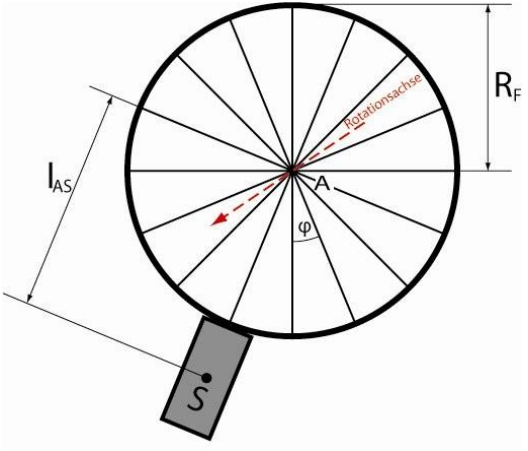
\includegraphics[scale=0.45]{./figure/speichenrad.png}
	\caption{Speichenrad mit Zylindermasse}
	\label{fig:rad}
\end{figure}

\end{multicols}
\end{document}